\documentclass[english]{textolivre}

% metadata
\journalname{Texto Livre}
\thevolume{18}
%\thenumber{1} % old template
\theyear{2025}
\receiveddate{\DTMdisplaydate{2024}{9}{30}{-1}}
\accepteddate{\DTMdisplaydate{2025}{1}{24}{-1}}
\publisheddate{\DTMdisplaydate{2025}{2}{25}{-1}}
\corrauthor{Lucio Agostinho Rocha}
\articledoi{10.1590/1983-3652.2025.54910}
%\articleid{NNNN} % if the article ID is not the last 5 numbers of its DOI, provide it using \articleid{} commmand 
% list of available sesscions in the journal: articles, dossier, reports, essays, reviews, interviews, editorial
\articlesessionname{articles}
\runningauthor{Rocha}
%\editorname{Leonardo Araújo} % old template
\sectioneditorname{Daniervelin Pereira}
\layouteditorname{Leonardo Araújo}

\title{An Evaluation of Machine Learning Approaches in Educational Environments: A Systematic Literature Review}
\othertitle{Uma Avaliação de Abordagens de Aprendizado de Máquina em Ambientes Educacionais: Uma Revisão Sistemática da Literatura}

\author[1]{Lucio Agostinho Rocha~\orcid{0000-0001-8804-8698}\thanks{Email: \href{mailto:luciorocha@utfpr.edu.br}{luciorocha@utfpr.edu.br}}}
\affil[1]{Universidade Tecnológica Federal do Paraná, Engenharia de Computação, Apucarana, PR, Brasil.}

\addbibresource{article.bib}

\usepackage{array,enumitem,longtable}

\begin{document}
\maketitle
\begin{polyabstract}
\begin{abstract}
The goal of this article is to investigate how methodologies
based on machine learning are being applied in educational environments
to enhance the quality of learning in graduation courses. The method is
presented through a systematic review of literature on the main
methodologies of systems based on artificial intelligence applied in
smart classrooms. The results indicate that in the popularization of
machine learning, the widespread use of these technologies presents new
challenges for educators as learning agents who investigate learning
strategies alongside their learners. The learning with these recent
technologies faces challenges regarding the veracity, soundness, and
quality of information. In the classroom, it is important to take into
account the legal aspects and ethics principles involved in these recent
machine learning advances. Besides, these issues involve how popular
platforms combine data from multiple sources to generate useful
information with reduced human intervention. Nowadays, society lives
connected to a myriad of interconnected computational devices. In this
sense, the classrooms are evolving into learning spaces where students
learn together in a collaborative way and shape soft-skills abilities,
such as communication, relationship, and collaboration.

\keywords{Educational research \sep Smart classroom \sep Machine
learning \sep Learning processes \sep Artificial Intelligence.}
\end{abstract}

\begin{portuguese}
\begin{abstract}
O objetivo deste artigo é investigar como metodologias baseadas
em aprendizado de máquina estão sendo aplicadas em ambientes
educacionais para melhorar a qualidade do aprendizado em cursos de
graduação. O método é apresentado através de uma revisão sistemática da
literatura das principais metodologias de sistemas baseados em
inteligência artificial aplicados em salas de aula inteligentes. Os
resultados indicam que na popularização do aprendizado de máquina, a
disseminação do uso dessas tecnologias apresenta novos desafios para
educadores como agentes de aprendizagem que investigam estratégias de
aprendizagem ao lado de seus aprendizes. A aprendizagem com essas
recentes tecnologias enfrenta desafios em relação à veracidade, solidez
e qualidade da informação. Na sala de aula, é importante levar em
consideração os aspectos legais e os princípios éticos envolvidos nesses
recentes avanços com aprendizado de máquina. Além disso, essas questões
envolvem como plataformas populares combinam dados de múltiplas fontes
para gerar conteúdo útil com reduzida intervenção humana. Nos dias
atuais, a sociedade vive conectada a uma miríade de dispositivos
computacionais interconectados. Nesse sentido, as salas de aula estão
evoluindo para espaços de aprendizagem onde estudantes aprendem juntos
de maneira colaborativa, e modelam habilidades de \emph{soft-skills},
tais como comunicação, relacionamento e colaboração.

\keywords{Pesquisa educacional \sep Sala de aula inteligente \sep
Aprendizado de máquina \sep Processos de aprendizagem \sep Inteligência
Artificial}
\end{abstract}
\end{portuguese}
\end{polyabstract}

\section{Introduction}\label{sec-intro}

The sustainability of education should foster ethical aspects reflected
in a healthy partnership between educators and their students. In
traditional education, the focus is on the average performance of
students \cite{Luan2021}, but this concept neglects personal learning
behaviors. It is a common issue that to follow individual learning
demands effort and time from both learners and educators. So, many
educators use information and communication technologies (ICT) to
improve the quality of their classes by automating many educational
tasks, such as tests and exams, to follow the continuous progress of
their students. The standardization of learning with automatic
tools may imply a reduction of creativity and diversity of
teaching methodologies, and auxiliary digital technologies could
increase the costs of effective learning. In a taylorist perspective, a
``shelf teacher'' appears to play a role in increasing productivity, but
in the constructivist theory, the importance of learning is revealed as
an active process based on personal experience and self-reflection
supported by experienced educators. In this sense, to effectively
improve the quality of education, it is essential to investigate the
incorporation of new digital technologies in classrooms.

In fact, smart campuses improve the quality of education with the
convergence of new digital technologies in the context of smart cities
to satisfy social needs \cite{ChamorroAtalaya2023}. Besides, systems
based on Artificial Intelligence (AI) have been applied in education
since the 1970s, and they are used as virtual pedagogical agents to
promote personalized learning, such as assessment and feedback.
Automated learning-based systems have gained importance mainly due to
their ability to solve non-trivial tasks, including solving math
formulas, producing texts and images, programming codes, and others.

In this article, the objective is to investigate how Machine Learning
(ML) and related methodologies for smart classrooms are being applied in
educational environments to improve the quality of learning in
graduation courses. In order to give a contextualization of this theme,
a systematic review of literature is presented in the following
sections. The relevance is to obtain insights into methodologies and
best practices that may be applied as guides to improve the quality of
education supported by recent digital technologies. This paper
summarizes some of the most relevant features of smart classrooms.

This article is structured as follows. The next section presents a
background of AI technologies applied in smart classrooms; Section \ref{sec-review}
presents a methodology of systematic review to select relevant articles
for this theme; Section \ref{sec-dis} discusses these latter results; finally,
Section \ref{sec-conc} does final considerations.


\section{Background}\label{sec-back}
According to \textcite{Shapiro2003}, Artificial Intelligence (AI) is a field of
computer science devoted to deal with computational aspects of
intelligent behavior. \textcite[p.~37]{Russel2021} define AI as a
system that performs correct actions based on rationality, and a system
is considered rational when it does the correct action based on its
available data. \textcite{Zhang2021} indicate that the main areas of
AI are the perception, the communication, the planning, the reasoning,
and the knowledge engineering. The term AI is defined as follows:

The term ``Artificial Intelligence'' (AI) was first mentioned by John
McCarthy in 1956 and refers to the ability of computer systems to
undertake human tasks (like learning and thinking) that frequently can
only be attained through human intelligence
\cite[p.~2]{Dimitriadou2023}.

Machine Learning (ML) is a knowledge area of AI that concentrates on
designing systems through algorithms that learn or improve their
performance based on the data they consume
\cite{Oracle2024, Eglite2022}. ML and AI are frequently presented
together, but they are not the same concept. In general, the two primary
ML algorithms that are frequently used are supervised and unsupervised
learning. The algorithms of supervised learning are trained with labeled
data sets and have a predefined output. The algorithm could use a
dictionary of fruit names to group labeled images, for instance. The
most common algorithms of supervised learning are linear regression and
logistic, multiclass classification, and support vector machines; 
but the algorithms for unsupervised learning utilize a different
approach. The system learns to identify processes and complex patterns
with minimal human intervention. This ML process involves training based
on unlabeled data sets or a predefined output. For instance, the
algorithm could group unlabeled images by their similarities with images
of fruits, and place them in specific groups, setting a new label for
each new group (e.g., a group of similar images of maces, a group of
similar images of strawberries, and so on). The common algorithms of
unsupervised learning include k-means, association rules, principal and
independent component analysis.

ML is being applied in smart classrooms, and this concept is evolving
over the years. \textcite{Yang2021} give to ``smart learning
environment'' a definition of an effective learning place that provides
appropriate resources and convenient interaction tools with automatic
record and evaluation of results. Additionally, \textcite{Dimitriadou2022} also define this concept as an integrated learning space that
combines emerging technologies. The personalized learning through
computational devices is meaningful to engage students in self-learning
according to their profile, needs, and interests. A recent approach
\cite{Luan2021} is to collect learning patterns to intervene properly
with teaching materials, considering the differences between learners.

It is important to consider the reliability, safety,
and implications of incorporating emergent digital technologies in
classrooms. The reliability in a sense of soundness of digital contents;
the safety in the sense of quality of information in the era of fast
widespread of unreliable information on digital media; and the
implications due to the effort to improve the abilities of thinking and
critical skills with these new technologies during classes.

\textcite{Chen2021} declare that AI applied in education has been
extensively used in online platforms, web-based chatbots, humanoid
robots, and computer programs. These authors also indicate that these
technologies may be applied to special education, performance
prediction, emotional detection, personalized learning, discourse
analysis, teaching evaluation, natural language processing, and
educational robots. In this sense, ethical issues need to be considered
about personnel data \cite{Pelletier2021}. For instance, the use of
these data, its access roles, security restrictions, storage, and the
duration of their availability.

The application of new emerging digital technologies in classrooms is
characterized by different definitions and terminology. According to
\textcite{Wang2023}, education systems based on AI are related with
emergent technologies. \textcite{ChamorroAtalaya2023} consider the term
Education 4.0 to describe educational practices based on competences and
supported by AI with exchange of knowledge in cloud environments. In
Education 4.0, intelligent educational environments shape professional
skills and social responsibility.

The emergence of AI technologies is associated with smart classrooms as
a complementary alternative to offer more creative and efficient
learning. Some of the main technologies in smart classrooms are
robotics, computer vision, augmented/virtual/mixed reality, active
methodologies, mobile devices, sensors, and computer vision-based
surveillance supported by e-learning platforms \cite{Dimitriadou2022}.
The role of teachers is to enhance the skills of their students through
new ubiquitous, social and mobile learning methodologies. The
combination of AI jointly of these emergent technologies shows that
smart classrooms are still evolving to be used during the learning
process. In smart classrooms, the students are encouraged to learn by
themselves and also bring their own devices to classes. Some authors
consider that big data and cloud computing, supported by additional
tools of speech recognition and deep learning, are the basis for the
effectivity of many smart classrooms. For instance, Gui (2020) does the
building of English teaching aided by neural networks to guide the
reform of foreign language education. This methodology can receive
various network resources and carry out characteristic data through deep
learning. \textcite{Li2023} also utilize big data sets to predict
the grades of English learners.

In addition to this, the advent of SARS-CoV-2 (COVID-19) impacted the
acceptance of online courses and provided opportunities to evaluate new
technologies in the graduate courses, especially in university settings,
when all teaching became virtual, testing the sustainability of
education systems. Another aspect is that inclusion, jointly with
equitative activities, should be offered in higher education to promote
sustainable possibilities \cite{Chai2024}. Although investments in
higher education brought interest in leverage AI science, learners were
impacted by restrictions in technological issues, connectivity, and
solitary learning. It is an empirical issue that many online courses
were shown by themselves to be inefficient to carry out the effective
personalized learning without the interaction with the human educator.
However, learning with ML systems was possible due to the explosion in
the volume of data during the second half of the 2000s and the
popularization of data capture through cheap devices.

For smart classrooms, it is possible to use ML algorithms with
structured data as databases and unstructured data as images, audio and
video to build decision-making systems to predict and classify data from
huge datasets. In these systems based on ML, pre-trained models are used
to find solutions that are not explicitly defined in the dataset
\cite{Shaik2022}. More specifically, the most common are those that use
ML to analyse, learn and apply classifying and prediction from datasets.
Deep learning holds multi-layer neural networks with
processing layers to train new concepts and link to previous. Recurrent
neural networks (RNNs) and gated recurrent units (GRUs) are examples of
techniques that apply deep learning to text classification. Other
examples are long short-term memory (LSTM) and convolutional neural
networks (CNNs) \cite{Shaik2022}.

In summary, most smart classrooms in higher education use blended
learning \cite{Chen2021} supported by a myriad of digital
technologies. In this sense, it is important to investigate how smart
environments are useful to improve learning in classrooms.


It is observed that the application of ML systems has shown its efficacy
and can potentially be applied jointly with active methodologies.
However, the use of these methodologies based on automated systems may
also be insufficient when learners demonstrate passive behavior during
the learning process. Besides, the environment of classrooms should be a
place of constant human interaction.

\begin{figure}[htbp]
\centering
\begin{minipage}{.75\textwidth}
  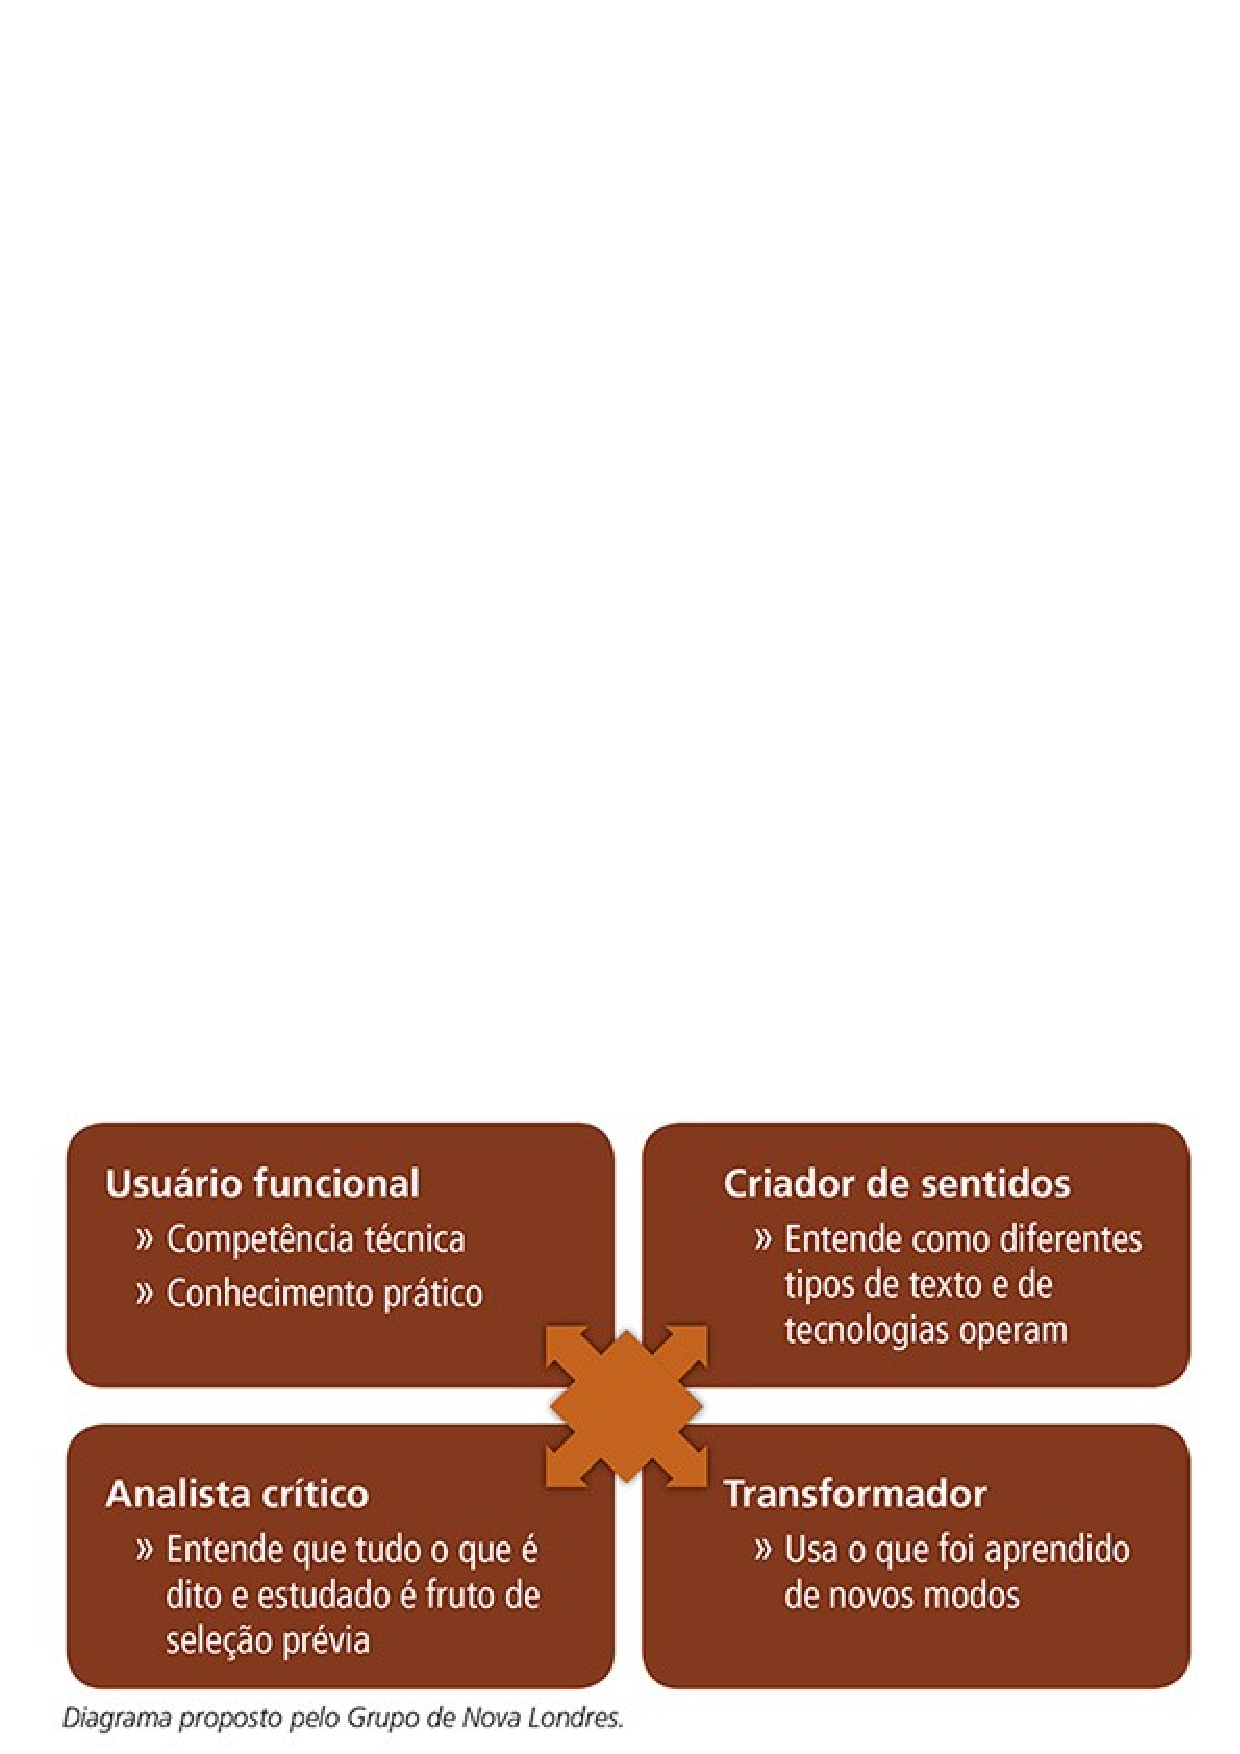
\includegraphics[width=\textwidth]{figure01.png}
  \caption{Flowchart of the Systematic Review.}
  \label{fig01}
  \source{Created by the author.}
\end{minipage}
\end{figure}


\section{Systematic Review of the Literature}\label{sec-review}

In this sense, it is fundamental to investigate how the application of
ML systems and related methodologies contributes to improve learning in
classrooms. The methodology employed in this article is based on the
Preferred Reporting Items for Systematic Reviews and Meta-Analysis
(PRISMA), which is a methodology commonly found in the literature
\cite{MontoyaRodriguez2023, Alfoudari2021, Shazli2023}. In this
systematic review, the research topics are identified, evaluated, and
analyzed. The proposed review is as follows: a) the definition of
research questions; b) the definition of search terms; c) the selection
of bibliographic bases; d) the definition of inclusion and exclusion
criteria for articles; e) the summary reading of these selected
references. In this systematic review, three steps were defined to
select articles: 1) Selection Phase: the search of papers according to
the selected bases; 2) Evaluation Phase: the filtering by relevance of
title, resume, keywords, and period starting from 2020; 3) Synthesis
Phase: the evaluation of these papers in both quantitative and
qualitative terms. \Cref{fig01} shows the steps followed in this study.

\begin{table}[ht]
\centering
\begin{threeparttable}
\caption{Criteria for the Eligibility.}
\label{tab01}
\begin{tabular}{
>{\raggedright\arraybackslash}p{0.5\textwidth} 
>{\raggedright\arraybackslash}p{0.5\textwidth}
}
\toprule
Items of Inclusion Criteria & Items of Exclusion Criteria \\
\midrule
\begin{enumerate}[label=\alph*)]
    \item The studies that address the concepts of the search string: (“artificial intelligence” OR “machine learning”) AND (“educational research” AND “smart classroom”).
    \item The articles written in English published in the last five years, starting from 2020 until the first half of 2024.
    \item The practical application of artificial intelligence to the improvement of learning in graduation courses.
\end{enumerate} &
\begin{enumerate}[label=\alph*)]
    \item The proposals and concepts not applied in the classroom;
    \item The papers without pedagogical analysis of artificial intelligence technologies in graduation courses.
\end{enumerate}
 \\
\bottomrule
\end{tabular}
\source{Created by the author.}
\end{threeparttable}
\end{table}

The research questions (RQ) are necessary to evaluate the references,
and they are presented in the following items:
\begin{itemize}
    \item[RQ 1]: What are the goals for using ML in the classroom?
    \item[RQ 2]: What methodologies are used in graduation courses?
    \item[RQ 3]: What ML softwares support this type of learning?
    \item[RQ 4]: What are the contents that have been developed?
\end{itemize}
The RQ 1 defines the objective of the article, as the focus is on ML
techniques for graduation courses; the RQ 2 identifies the methodology;
the RQ 3 identifies the ML softwares that were used for learning;
finally, the RQ 4 describes the developed contents in the classroom.

These research questions were used to define the following keywords:
artificial intelligence, machine learning, educational research, and
smart classroom. Then, the search string is: (``artificial
intelligence'' OR ``machine learning'') AND (``educational research''
AND ``smart classroom''). This search string was submitted to these
digital bibliography catalogues: IEEE Xplore, Elsevier Scopus, DOAJ
(Directory of Open Access Journals), and reviewed articles found by
Google Scholar. These databases are considered reputable in terms of
research quality. The inclusion criteria (IC) are: a) the studies that
address the concepts of the search string; b) the English articles
published in the last five years, starting from 2020 until the first
semester of 2024; c) the practical application of AI to the improvement
of learning in graduation courses. The exclusion criteria (EC) are: a)
the proposals and concepts not applied in the classroom; b) the papers
without pedagogical analysis of AI technologies in graduation courses.
These criteria are summarized in \Cref{tab01}.

\Cref{fig02} shows the obtained articles by year. Since 2020, there are many
researches related to the inclusion of AI in classrooms, and this issue
is shown in the figure. \Cref{tab02} summarizes the obtained articles in the
Selection phase.


\begin{figure}[htbp]
\centering
\begin{minipage}{.75\textwidth}
  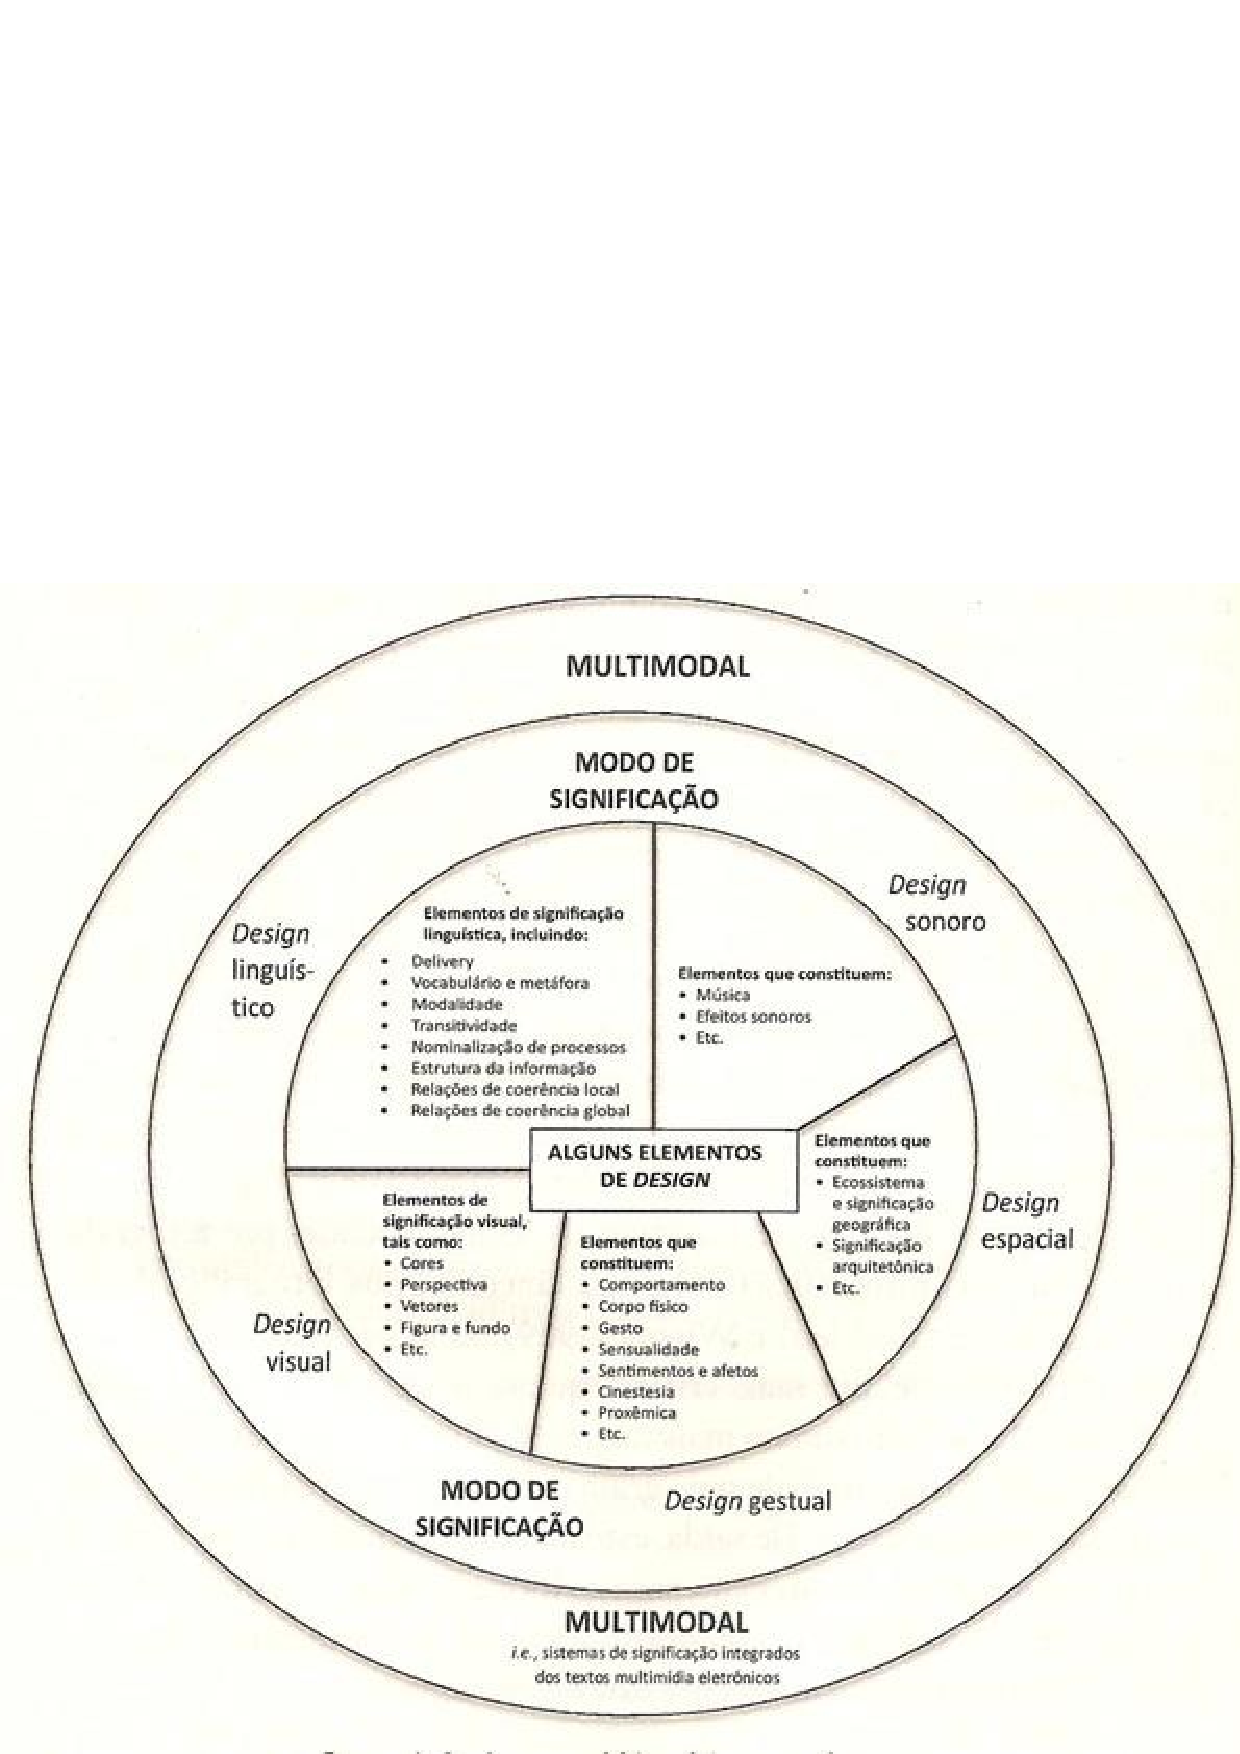
\includegraphics[width=\textwidth]{figure02.png}
  \caption{Selection Phase: Articles starting from 2020.}
  \label{fig02}
  \source{Created by the author.}
\end{minipage}
\end{figure}


\begin{table}[ht]
\centering
\begin{threeparttable}
\caption{Systematic Review of the Literature.}
\label{tab02}
\begin{tabular}{
>{\raggedright\arraybackslash}p{0.22\textwidth} 
>{\raggedright\arraybackslash}p{0.22\textwidth} 
>{\raggedright\arraybackslash}p{0.22\textwidth} 
>{\raggedright\arraybackslash}p{0.22\textwidth}
}
\toprule
Catalogue Sources & Step 1 Selection Phase: Inclusion criteria & Step 2 Evaluation Phase: Exclusion criteria (a) & Step 3 Synthesis Phase: Exclusion criteria (b) \\
\midrule
IEEE & 72 & 32 & 26 \\
Elsevier & 9 & 2 & 2 \\
DOAJ & 9 & 5 & 5 \\
Google Scholar & 78 & 42 & 40 \\
Total & 168 & 81 & 73 \\
\bottomrule
\end{tabular}
\source{Created by the author. This dataset is available at: \url{https://osf.io/5kxzs}.}
\end{threeparttable}
\end{table}

The visualization by category including the article surveys is given in
\Cref{fig03}. In this figure the obtained articles may be included in more
than one category. The next section discusses these latter results.




\section{Discussion of the Results}\label{sec-dis}
The previous section results allow answers to the research questions. In
the evaluation of the RQ1, the selected articles indicate the
possibility of improving classrooms with AI-based systems and their
related technologies. However, a further discussion is conducted in the
following to clarify the reproducibility of these innovations and avoid
the higher costs of non-sustainable approaches.


\begin{figure}[htbp]
\centering
\begin{minipage}{.75\textwidth}
  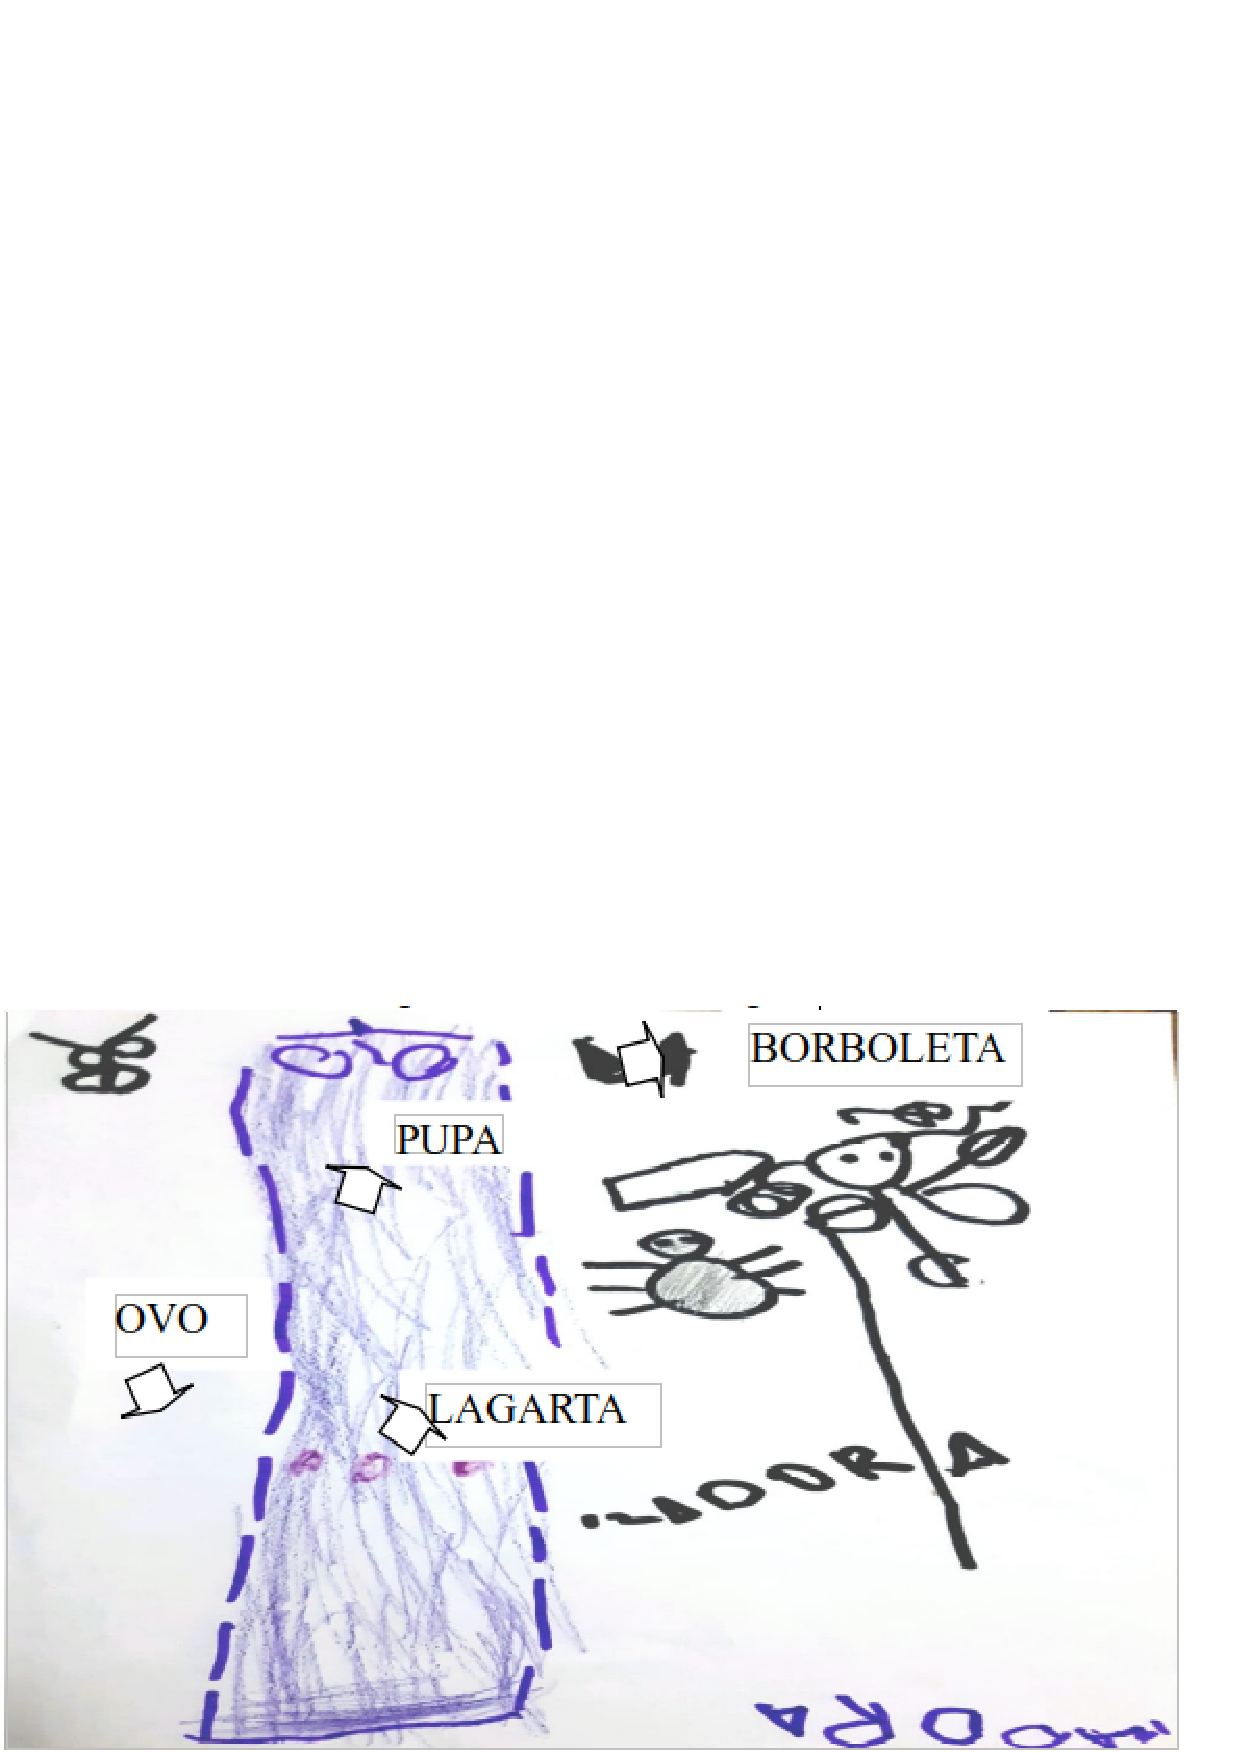
\includegraphics[width=\textwidth]{figure03.png}
  \caption{Classification of Methodologies for Smart Classrooms.}
  \label{fig03}
  \source{Created by the author.}
\end{minipage}
\end{figure}


Related to the RQ2 and RQ3, \Cref{tab03} summarizes the main methodologies
and software tools for application in smart classrooms. Some
similarities are observed that permit to categorize them as follows:
E-learning platforms; NLP; mixed/virtual/augmented reality;
gamification; big data analysis; performance prediction; and
monitoring/surveillance with computer vision. These categories are basic
and frequently interrelated, and aim to identify how research will
contribute to the creation of a smart classroom. As shown in \Cref{fig03},
these categories frequently appear together as keywords, with the
exception of NLP and gamification categories, which appear in minor
occurrences.

This review of the literature revealed contributions to the learning in
classrooms supported by AI-based systems and newer digital technologies.
\Cref{tab03} emphasizes the main methodologies used in the implementations of
smart classrooms excluding surveys, as the latter describes multiple
methodologies.

\clearpage
\begin{longtable}{@{}
>{\raggedright\arraybackslash}p{0.315\textwidth} 
>{\raggedright\arraybackslash}p{0.315\textwidth} 
>{\raggedright\arraybackslash}p{0.315\textwidth} 
@{}}
\caption{Methodologies and Software Tools of Smart Classrooms.}
\label{tab03}
\\
\toprule 
Methodology & Software Tools & Smart Classrooms \\
\midrule
1. Massive Open Online Courses (MOOCs) and Online platforms for
e-learning. & a) Google Classroom; b) Canvas; c) Blackboard; d) Moodle;
e) BigBlueButton; f) chat online meeting like videoconference (For
example: Zoom, WebEx, Google Meeting, Skype, Microsoft Teams); g) online
quizzes; h) YouTube; i) Facebook; j) 2U; k) Loud Cloud; l)
Adaptcourseware; m) Anewspring; n) customized e-learning platforms based
on Fog/Cloud Computing and others. & Zhang \emph{et al}. (2022),
Bhatnagar; Sharma (2022), Shaik \emph{et al}., 2022; Wu \emph{et al}.
(2021); Syzdykbayeva; Baikulova; Kerimbayeva (2021). \\
2. Natural Language Processing (NLP) & a) Chatbots; b) chatGPT, and
others. & Shaik \emph{et al}., (2022); Tang; Li (2023). \\
3. Virtual/Augmented Mixed Reality & a) Neural networks; b) Markov
chains; c) deep learning frameworks (e.g. Caffe); d) trained based
models from public datasets; e) OpenPose; f) Tensorflow, and others. &
Zhang \emph{et al}. (2020), Haghighi \emph{et al}. (2021). \\
4. Gamification & a) Learning management systems (LMS); b) immersive
reality; c) simulations with serious game; d) interactive media; e)
HelloTalk; f) Lingualeo; g) Hello English; h) Memrise; i) Duolingo; j)
browser games and others. & Dahalan; Alias; Shaharom (2023),
Syzdykbayeva; Baikulova; Kerimbayeva (2021), Zhu; Guo; Yang (2023). \\
5. Big Data Analysis & a) Citespace; b) VOSviewer; c) Bibliometrix; d)
Pytorch; e) word clouds; f) Spssau; g) Ucinet; h) Netdraw; i) datasets
from questionnaires; j) public facial expression datasets; k) ML
algorithms, and others. & Bhatnagar; Sharma (2023), Chai; Ye (2024),
Bansal; Ahmed (2023), Madhani; Shah; Swarnalatha \emph{et al}. (2022),
Li; Yao (2023). \\
6. Performance Prediction & a) Random Forest (RF); b) K-nearest
neighbors (KNN); c) artificial neural networks (ANN); d) support vector
machine (SVM); e) Gradient Boosted Regression Trees (GBRT); f) Long
Short-Term Memory (LSTM); and others. & He; Hu (2022), Luan; Tsai
(2021), Zhao \emph{et al}. (2020), Zhao \emph{et al}. (2022), Wu
\emph{et al}. (2021). \\
7. Monitoring and Surveillance with Computer Vision & a) Computer vision
algorithms such as YOLO, R-CNN series, etc.; b) recording softwares, and
others. & Pang; Lai; Zhang \emph{et al}. (2023), Song; Zhao; Xiong
\emph{et al}. (2022), Shanshan; Hui; Liqiao (2024). \\
\bottomrule
\end{longtable}

Related to the RQ4 that describes the contents developed in the
classroom, it is observed that there are few evaluations by ethical
committees of research regarding how changes will be implemented in
classrooms. Besides, most of the articles obtained do not consider
feedback from their students regarding how AI-based systems effectively
contribute or not to their performance. In this sense, qualitative
feedback from these students would be important to complement the
statistical results concerning the effort to perform lessons, the
duration to deliver tasks, the motivation of using automated learning
systems, and others. In order to complement the answer of these research
questions, a discussion is done as follows.

\begin{enumerate}
    \item Massive Open Online Courses (MOOCs) and Online platforms for
  e-learning: many online platforms for e-learning are publically
  available \cite{Zhang2022,Shaik2022,Wu2021,Bhatnagar2023,Syzdykbayeva2021}, and they have been the most utilized alternative to decrease
  weakness of teaching after the COVID-19 pandemic. In addition to this,
  the transition from in-person to online compelled educators to adopt
  systems that they were not prepared for \cite{Pokhrel2021}. One of
  the major challenges of online classes was the absence of fundamental
  requirements for quality learning, such as soft-skills gained by
  interpersonal relationship, communication abilities, expertise with
  information and communications technology, with the lack of adequate
  physical space for classes compelling emotional distress, for
  instance. The widespread dissemination of self-learning through large
  Internet resources has shown the need for an educator to properly
  guide problem-solving activities. For smart classrooms, \textcite{Zhang2022} also indicate the possibility of performing empirical
  analysis as an educational research method to capture teaching
  situations. This method has the potential to offer effective
  personalized feedback.
  \item Natural
Language Processing (NLP): this category is cited less frequently in the
results, and one of the reasons is probably its relative new adoption in
e-learning platforms, associated with its inherent difficulty in
creating educational content. NLP is widely used for opinion mining.
\textcite{Shaik2022} reveal that NLP is useful to evaluate feedback from
students without human intervention. Besides, AI in education can
collect data non-explicitly given by the student and adjust the teaching
approach through adaptive learning platforms. These systems come to give
an adaptive learning system based on students' background by continuous
monitoring and tracking of students' textual feedback. Additionally,
online applications like Turnitin aim to check plagiarism, typographical
and grammatical errors \cite{Shaik2022}. \textcite{Tang2023} use ChatGPT
to adjust teaching contents with personalized learning. Chatbots use NLP
and Deep Neural Networks (DNN) to give predictions, recognize speech and
respond properly. Chatbots have become a recent option for personal
assistance and tutoring in classes, which can be used to answer
questions, distribute material, watch videos, and play games.
  \item Virtual/Augmented/Mixed Reality: smart classrooms with immersive
  environments are the combination of virtual/augmented/mixed reality
  devices that may potentially contribute to greater knowledge
  retention, improve problem-solving skills, and promote more engaging
  experiences \cite{Dimitriadou2022}. \textcite{Zhang2021} also
  highlight the possibility of investigating students' behavior, and
  \textcite{Haghighi2021} the possibility of automating the face
  recognition for recording classes. Unfortunately, some restrictions
  are related to the relative weaknesses of content, the difficulties of
  producing virtual/augmented content, and the high costs of acquiring
  specific devices.

  \item Gamification: this category is also cited less frequently in the
  results, and two of the probable reasons are the lack of acceptance by
  educators and the quality of educational content. Gamification has the
  potential of improving the educational experience by increasing
  motivation, engagement, and academic accomplishment
  \cite{Dahalan2024}. \textcite{Syzdykbayeva2021}
  also indicate the possibility of gamification for learning foreign
  languages. Teachers can provide teaching materials, AI extracts the
  key concepts, and the system generates questions and answers. \textcite{Zhu2023} indicate that 21st century skills should involve
  high-order skills which encompass creativity and critical thinking,
  for example. In this sense, these authors indicate the possibility of
  utilizing digital game-based assessment to engage behaviors by
  constructing game contexts through distinct game genders. These
  digital games contain incentives to enhance engagement and motivation,
  can capture the interactions yielded during the game, and allow
  reproducibility of the individual process of problem-solving to
  support interventions.

  \item Big Data Analysis: many authors combine big data sets from
  different sources and perform the analysis of these data sets with ML
  algorithms \cite{Bhatnagar2023,Chai2024,Bansal2023,Madhani2022,Li2023}. In
  fact, there are many different alternatives of data analysis for smart
  classrooms: text mining, sentiment, social network, statistical,
  facial, IoT data, and others. \textcite{Zhu2023} indicate two
  main categories for data analysis that are supervisioned models and
  statistical analysis. A possibility for supervisioned models is to
  include in ML modeling knowledge, skills, and affections of students
  as labels. Then, the relationship between the labeled data can be
  trained to achieve predictions on new outcomes. The most common
  technique of data analysis of supervisioned models is linear
  regression, and the most common technique of data analysis of
  statistical results is the correlation analysis. 
  IoT offers a myriad of devices connected to the Internet. The most
  common applications are real-time monitoring, safe infrastructure,
  building administrative task automation, e-contents, and also online
  live sessions within the university campuses, although many of these
  devices leak in interoperability \cite{Bhatnagar2023}. IoT devices
  may potentially acquire real data and facts to feed customized deep
  learning with AI, and generate a Fog-IoT portfolio designed for
  private clouds by universities \cite{Bhatnagar2023}.

  \item Performance Prediction: many ML algorithms have been used to
  predict academic performance and admission decision \cite{Zhu2023}.
  \textcite{He2022} affirm that the performance prediction supported by
  deep learning comes jointly with the advent of the fourth industrial
  revolution. These authors believe that deep learning should focus in
  comprehension, analysis, application, and evaluation, in contrast with
  superficial learning of memorization. In fact, smart classrooms should
  overcome simple mechanical memorizing in contrast with a high level of
  cognition. \textcite{Zhu2023} indicate that self-reported
  surveys ignore the thinking process, and negligence aspects of
  high-order skills. The self-report aims to evaluate how well the
  students do tasks. A standardized test is considered highly reliable
  and valid where the students have to answer
  a pre-defined set of questions. However, in terms of methodology,
  tests with questionnaires leak the capture of the thinking process
  during learning, and make it difficult to avoid anxiety and to foster
  engagement, problem-solving abilities, and memory performance.
  Commonly, only the final score obtained is evaluated. As a
  consequence, if a student gives a wrong answer, the thinking process
  is not evaluated. In addition to this, many authors \cite{He2022},
  \textcite{Luan2021,Zhang2021,Zhang2022,Wu2021} propose methodologies to improve learning during the
  classes supported by ML and deep learning tools for data analysis.

  \item Monitoring and Surveillance with Computer Vision: \textcite{Dimitriadou2022} indicate that computer vision-based surveillance and
  smart environments contribute to delivering efficient classes.
  Computer vision is often used to reduce the time for verifying the
  presence and detecting behaviors using facial identification
  technologies, such as high anxiety, uncomfortable situations, and
  concentration levels. A similar approach is proposed by \textcite{Shanshan2024} to build a teaching system based on face
  recognition, as an alternative to observing the behavior of students
  in classrooms. Automated methods for behavior analysis are widely used
  in smart classrooms to recognize student actions, and prevent mental
  and physical injuries. \textcite{Dimitriadou2022} also indicate
  that students can positively interact with educational AI-based
  robots, which can contribute to improve the learner's knowledge.
\end{enumerate}




\section{Conclusion}\label{sec-conc}
Nowadays, AI poses many challenges to educators, but it is evident that
this technology cannot replace human soft-skills abilities, such as
communication, organization, leadership, team formation, adaptation,
creativity, interpersonal relationship, and also the critical thinking
abilities of judgment and decision-making. This underscores the
importance of evaluating before using auto-generated answers.
AI-generated content and its inherent ambiguity further emphasize the
importance of critical thinking and judgment \cite{cao2023navigating}. AI tools,
as chatbots for instance, may be an alternative to solve repetitive
tasks of specific lessons and tests, but are insufficient to perform
tasks that need immaterial abilities for learning, including improving
communication, enhancing expressiveness, working with teams,
brainstorming, and developing proposals, to cite a few.

\textcite{Dimitriadou2022} give insights into the strengths of AI to
give adaptive modes of interaction, personalized feedback and advice.
However, many weaknesses were also observed, such as feelings of
disengagement from learning. In fact, Vygotsky \cite{ODonnell1999}
considers learning as a cognitive process that needs human interaction
to be consolidated, and not only to retain information more easily. In
addition to this, according to \textcite{Yang2021}, the Internet connects
people, but these connections are not necessarily indicative of
effective learning. Many online platforms have the weakness of high
costs for maintaining their infrastructure and to keep their services,
which is almost impossible to be sustainable in the long term for some
AI tools, mainly when big datasets are extracted from multiple sources.
\textcite{Dimitriadou2022} also reveal threats, such as the negative
impact of insert failures and/or non-confidence results during the
training process of systems based on ML, reducing the quality of the
teaching process. Besides, the high amount of individual data needs an
effective role for security and privacy, which is almost impossible to
maintain in some schools without rigorous ethical partnerships.

García-Tudela, Prendes-Espinosa and Solano-Fernández (2023) emphasize
educational environments to develop competences, commonly known as
soft-skills. Besides, they indicate greater prominence to the
personalization of teaching automatically with integration of emerging
technologies of AI, learning analytics, sensors and others. \textcite{Mustafa2022} consider the importance of putting the learner as the main
actor of the learning process. In addition to this, active methodologies
such as flipped classrooms promote events that traditionally are taken
inside the classroom, and that now can take place outside of this
environment. Some of these strategies involve virtual and remote
classrooms to be on online courses and to interact with emerging
technologies, such as AI. However, some authors \cite{Dimitriadou2022}
indicate that some recent digital technologies have also been proven to
enforce isolation, and impede students in rural areas or with
disabilities.

Finally, the emergence of many online courses supported by automated
tools brings issues about how this excessive amount of information is
being absorbed by students. The proposal of ``learn by yourself'' raises
some issues about how the quality of this methodology impacts
interpersonal relationship in-class and remotely. In fact, \textcite{farahani2018towards} highlighted that prolonged use of the computer may cause
corporal issues, such as neck strain and visual discomfort. Technology
has been identified as a cause of depression due to
people\textquotesingle s increased use of technology and decreased
social interaction. Besides, physical and mental health are also
affected \cite{brohi2023exploring}. The dependency on automated tools may lead
to a decrease in critical thinking and a growing spread of
misinformation.


\section*{Acknowledgements}
The author acknowledges the Federal University of Technology -- UTFPR
campus Apucarana -- for supporting this research.

\section*{Conflict of Interest}
The author declares that there is no conflict of interest.

\printbibliography\label{sec-bib}
%conceptualization,datacuration,formalanalysis,funding,investigation,methodology,projadm,resources,software,supervision,validation,visualization,writing,review
\end{document}
